\textit{Le but de ce TP est d'implémenter deux algorithme de résolution du problème de flot maximum : l'algorithme d'Edmonds-Karp et l'algorithme de Dinic. Nous commencerons par spécifier les fonctionnalités que devra implémenter notre programme, puis nous détaillerons la manière dont ces fonctionnalités ont été développées. Une troisième partie sera consacrée aux tests effectués sur les deux algorithmes ainsi qu'à l'analyse des résultats.}

\section{Spécification fonctionnelles}

\subsection{Résolution du problème de flot maximum}

Le programme doit être capable de :
\begin{itemize}
\item générer et d'actualiser les graphes d'écarts successifs
\item calculer la valeur du flot obtenu à partir du graphe d'écart final
\item résoudre le problème de flot maximum en suivant l'algorithme d'\textbf{Edmonds-Karp}
\item résoudre le problème de flot maximum en suivant l'algorithme de \textbf{Dinic}
\item retourner la solution de manière exploitable pour l'analyse
\end{itemize}

Il faudra veiller à conserver les complexités des deux algorithmes, notamment en prenant garde aux structures de données et librairies utilisées.

\subsection{Génération aléatoire d'un réseau de transport}

La génération aléatoire de graphes de type réseau de transport permettra de tester les deux algorithmes. Il faudra veiller à ce que le graphe respecte les conditions d'un réseau de transport notamment la possession d'une source et d'un puits, la pondération des arcs (capacités), et assurer la connexité du graphe. La génération de ce réseau de transport devra être paramétrable selon la taille (nombre de sommets) et la couverture (nombre d'arcs).

\section{Spécification technique}

\subsection{Programmation C++}
Parce qu'il s'agit d'un bon compromis entre langage orienté objet et langage de bas niveau, nous avons choisi de développer cette application en C++. Nous pourrons ainsi abstraire la gestion des graphes (notamment des structures de données) dans nos algorithmes, tout en gardant la possibilité d'optimiser le code grâce à la flexibilité du langage C.

\subsection{Structures de données}

Plusieurs structures de données sont possibles. Nous avons choisi d'implémenter une représentation par listes d'adjacences et une autre par matrice d'adjacences.
\begin{description}
\item[Listes d'adjacences] : chaque sommet possède la liste de ses voisins. Ces listes ont l'avantage d'allouer de la mémoire uniquement lorsqu'une information doit être stockée. 
\item[Matrice d'adjacences] : la mémoire allouée pour cette structure de données ne dépend que du nombre de sommets ($n^2$). Cette structure a l'avantage d'offrir un accès direct à un arc pour deux sommets donnés.
\end{description}

Dans un but d'optimisation mémoire, on utilise en général des listes d'adjacences lorsque l'on travail sur des graphes peu denses. En effet, la taille allouée par cette structure de données étant directement dépendante du nombre d'arcs, elle est donc réduite par rapport aux matrices d'adjacences. Sur des graphes très dense, on utilisera plutôt des matrice d'adjacences, permettant un accès aux données plus rapide. 

Ce choix s'effectue en général en fonction des ressources matériels disponibles.

\subsection{Modélisation}
Dans un but d'abstraction de la structure de donnée, nous avons choisi de créer une classe abstraite \texttt{AbstractGraph} dont deux classes fille héritent. Un graphe peut donc être de type \texttt{AdjacencyListGraph} ou \texttt{MatrixGraph}.
\begin{figure}[t]
\begin{center}
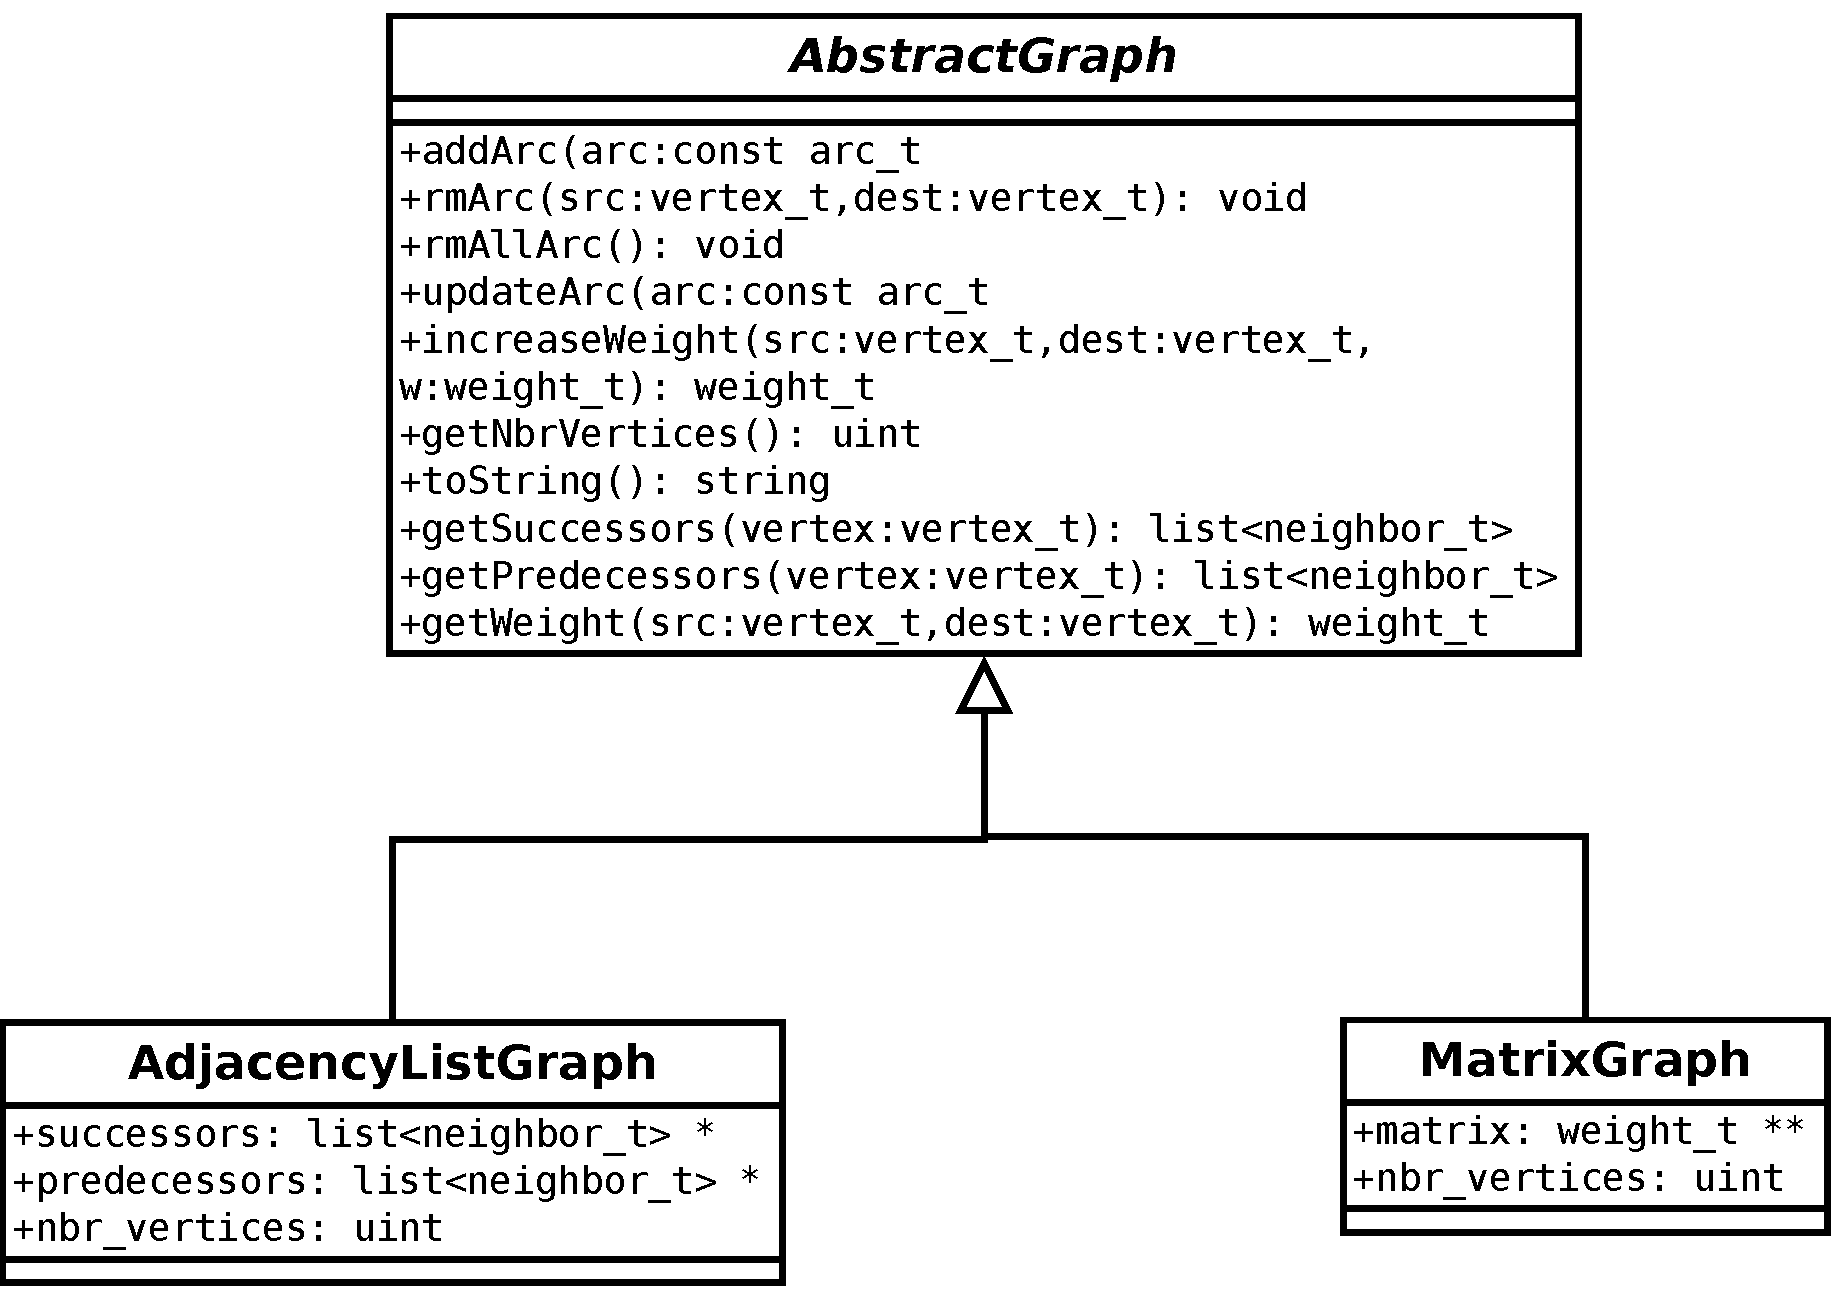
\includegraphics[width=\textwidth]{files/diag_class}
\end{center}
\caption{Diagramme de classes.}
\end{figure}

\FloatBarrier

\subsubsection{Classe \texttt{AbstractGraph}}

Header de la classe \texttt{AbstractGraph}

\lstinputlisting[language=C++,morekeywords={}]{./sources/AbstractGraph}

\subsubsection{Classe \texttt{AdjacencyListGraph}}
Cette classe représente un réseau de transport sous la forme
de deux listes d'adjacences : une représente les 
successeurs d'un sommet, l'autre les prédécesseurs.

Ce doublon d'information permet d'accélérer l'accès aux voisins d'un sommet, notamment à ces prédécesseurs. En effet, cette méthode nous permet d'accéder aux prédécesseurs directement (complexité de $O(m)$) alors que l'accès via la liste des successeurs implique une recherche des arcs pour chaque sommet (complexité de $O(nm)$).

Ces doubles listes d'adjacences nous assurent un gain de performances en terme de rapidité, qui se fait au détriment de la quantité de mémoire utilisé, qui se trouve doublée.

Header de la classe \texttt{AdjacencyListGraph}

\lstinputlisting[language=C++,morekeywords={}]{./sources/AdjacencyListGraph}


\subsubsection{Classe \texttt{MatrixGraph}}

Header de la classe \texttt{MatrixGraph}

\lstinputlisting[language=C++,morekeywords={}]{./sources/MatrixGraph}


\section{Tests \& résultats}
bla
\subsection{Méthode de test}

\subsection{Analyse des résultats}

///////////////////////////////////////////////////////////////////////////////////////

\subsection{Structures}

La représentation des 

\begin{verbatim}
typedef int weight_t;
typedef uint vertex_t;

typedef struct
{
  vertex_t u;
  vertex_t v;
} edge;

typedef struct
{
  vertex_t vertex_src;
  vertex_t vertex_dest;
  weight_t weight;
} arc_t;

typedef struct
{
  vertex_t vertex;
  weight_t weight;
} neighbor_t;
  
typedef list<vertex_t> path_t;

\end{verbatim}


\subsection{Génération aléatoire d'un graphe}

\begin{verbatim}
/**
 * A random flow network generator
 * Attention si le graph passé en paramètre contient des arcs ceux-ci seront
 * supprimé.
 * @param graph une référence vers un graph initialiser avec un nombre de sommets
 * @param rate la proportion d'arcs à ajouter au graphe en pourcentage par rapport au graphe complet.
 * @param min_weight valuation minimal des arcs
 * @param max_weight valuation maximal des arcs
 */
void
flowNetworkGenerator(AbstractGraph& graph, float rate, uint min_weight = 1,
    uint max_weight = 1);

\subsection{Fonctions générales}

/**
 * Cette procédure génère une chaîne de caractères représentant l'affichage
 * de la valeur total du flot sur le réseau de transport ainsi que la valeur
 * du flot sur chaque arc.
 * @param flow_network le réseau de transport
 * @param residual_network le graphe d'écart associé
 */
string
flowToString(const AbstractGraph& flow_network,
    const AbstractGraph& residual_network);



\subsection{Edmonds-Karp}

/**
 * Cette fonction retourne le plus court chemin en nombre d'arcs depuis
 * le sommet start jusqu'au sommet end
 * @param g un graphe
 * @param start le sommet de départ
 * @param end le sommet d'arriver
 * @return le plus court chemin en nombre d'arcs de start à end
 */
path_t
leastArcsPath(AbstractGraph &g, vertex_t start, vertex_t end);

/**
 * Cette fonction retourne la plus petite valuation présente sur un chemin 
 * donné dans un graphe
 * @param g un graphe
 * @param path une chemin dans g
 * @return la plus petite valuation présente sur le chemin path dans g 
 */
weight_t
lightestArc(AbstractGraph& g, path_t path);

/**
 * Cette fonction converti un chemin en chaîne de caractère dans un but d'affichage
 * @param path le chemin
 * @param g le graphe
 */
string
pathToString(path_t path, const AbstractGraph& g);

/**
 * Mise à jour du graphe d'écart depuis un chemin et la valeur du flot à ajouter
 * sur ce chemin
 * @param le graphe de couche
 * @param p le chemin
 * @param k la valeur du flot à ajouter
 */
void
updateResidualNetwork(AbstractGraph& residualNetwork, path_t p, uint k);


/**
 * algorithme d'Edmonds-Karp
 * @param flow_network le réseau de transport
 * @param src le sommet source
 * @param dest le puit
 * @return le graphe d'écart final
 */
AdjacencyListGraph
edmondsKarp(const AbstractGraph& flow_network, vertex_t src, vertex_t dest);

\end{verbatim}

\subsection{Dinic}

\begin{verbatim}
/**
 * Mise à jour du graphe d'écart depuis un flot
 * @param residual_network le graphe de couche
 * @param p le flot
 */
void
updateResidualNetwork(AbstractGraph& residual_network, AbstractGraph& flow);

/**
 * Génération du graphe de couche associé au réseau de transport
 * @param residual_network le graphe d'écart
 * @param src la source
 * @param dest le puit
 * @return le graphe de couche
 */
LevelGraph
generateLevelGraph(const AbstractGraph& residual_network, vertex_t src,
    vertex_t dest);

/**
 * Calcul du flot bloquant
 * @param level_graph le graphe de couche
 * @param src la source
 * @param dest le puit
 * @return un flot bloquant
 */
AdjacencyListGraph
blockingFlow(LevelGraph& level_graph, vertex_t src, vertex_t dest);


/**
 * algorithme de Dinic
 * @param flow_network le réseau de transport
 * @param src le sommet source
 * @param dest le puit
 * @return le graphe d'écart final
 */
AdjacencyListGraph
dinic(const AbstractGraph& graph, vertex_t src, vertex_t dest);

\end{verbatim}